%File: anonymous-submission-latex-2025.tex
\documentclass[letterpaper]{article} % DO NOT CHANGE THIS
\usepackage{aaai25}  % DO NOT CHANGE THIS
\usepackage{times}  % DO NOT CHANGE THIS
\usepackage{helvet}  % DO NOT CHANGE THIS
\usepackage{courier}  % DO NOT CHANGE THIS
\usepackage[hyphens]{url}  % DO NOT CHANGE THIS
\usepackage{graphicx} % DO NOT CHANGE THIS
\urlstyle{rm} % DO NOT CHANGE THIS
\def\UrlFont{\rm}  % DO NOT CHANGE THIS
\usepackage{natbib}  % DO NOT CHANGE THIS AND DO NOT ADD ANY OPTIONS TO IT
\usepackage{caption} % DO NOT CHANGE THIS AND DO NOT ADD ANY OPTIONS TO IT
\frenchspacing  % DO NOT CHANGE THIS
\setlength{\pdfpagewidth}{8.5in} % DO NOT CHANGE THIS
\setlength{\pdfpageheight}{11in} % DO NOT CHANGE THIS
%
% These are recommended to typeset algorithms but not required. See the subsubsection on algorithms. Remove them if you don't have algorithms in your paper.
\usepackage{algorithm}
\usepackage{algorithmic}

% user added package
\usepackage{amsmath}
\usepackage{amssymb}
\usepackage{booktabs}
\usepackage{subcaption}

%
% These are are recommended to typeset listings but not required. See the subsubsection on listing. Remove this block if you don't have listings in your paper.
\usepackage{newfloat}
\usepackage{listings}
\DeclareCaptionStyle{ruled}{labelfont=normalfont,labelsep=colon,strut=off} % DO NOT CHANGE THIS
\lstset{%
	basicstyle={\footnotesize\ttfamily},% footnotesize acceptable for monospace
	numbers=left,numberstyle=\footnotesize,xleftmargin=2em,% show line numbers, remove this entire line if you don't want the numbers.
	aboveskip=0pt,belowskip=0pt,%
	showstringspaces=false,tabsize=2,breaklines=true}
\floatstyle{ruled}
\newfloat{listing}{tb}{lst}{}
\floatname{listing}{Listing}
%
% Keep the \pdfinfo as shown here. There's no need
% for you to add the /Title and /Author tags.
\pdfinfo{
/TemplateVersion (2025.1)
}

% DISALLOWED PACKAGES
% \usepackage{authblk} -- This package is specifically forbidden
% \usepackage{balance} -- This package is specifically forbidden
% \usepackage{color (if used in text)
% \usepackage{CJK} -- This package is specifically forbidden
% \usepackage{float} -- This package is specifically forbidden
% \usepackage{flushend} -- This package is specifically forbidden
% \usepackage{fontenc} -- This package is specifically forbidden
% \usepackage{fullpage} -- This package is specifically forbidden
% \usepackage{geometry} -- This package is specifically forbidden
% \usepackage{grffile} -- This package is specifically forbidden
% \usepackage{hyperref} -- This package is specifically forbidden
% \usepackage{navigator} -- This package is specifically forbidden
% (or any other package that embeds links such as navigator or hyperref)
% \indentfirst} -- This package is specifically forbidden
% \layout} -- This package is specifically forbidden
% \multicol} -- This package is specifically forbidden
% \nameref} -- This package is specifically forbidden
% \usepackage{savetrees} -- This package is specifically forbidden
% \usepackage{setspace} -- This package is specifically forbidden
% \usepackage{stfloats} -- This package is specifically forbidden
% \usepackage{tabu} -- This package is specifically forbidden
% \usepackage{titlesec} -- This package is specifically forbidden
% \usepackage{tocbibind} -- This package is specifically forbidden
% \usepackage{ulem} -- This package is specifically forbidden
% \usepackage{wrapfig} -- This package is specifically forbidden
% DISALLOWED COMMANDS
% \nocopyright -- Your paper will not be published if you use this command
% \addtolength -- This command may not be used
% \balance -- This command may not be used
% \baselinestretch -- Your paper will not be published if you use this command
% \clearpage -- No page breaks of any kind may be used for the final version of your paper
% \columnsep -- This command may not be used
% \newpage -- No page breaks of any kind may be used for the final version of your paper
% \pagebreak -- No page breaks of any kind may be used for the final version of your paperr
% \pagestyle -- This command may not be used
% \tiny -- This is not an acceptable font size.
% \vspace{- -- No negative value may be used in proximity of a caption, figure, table, section, subsection, subsubsection, or reference
% \vskip{- -- No negative value may be used to alter spacing above or below a caption, figure, table, section, subsection, subsubsection, or reference

\setcounter{secnumdepth}{0} %May be changed to 1 or 2 if section numbers are desired.

% The file aaai25.sty is the style file for AAAI Press
% proceedings, working notes, and technical reports.
%

% Title

% Your title must be in mixed case, not sentence case.
% That means all verbs (including short verbs like be, is, using,and go),
% nouns, adverbs, adjectives should be capitalized, including both words in hyphenated terms, while
% articles, conjunctions, and prepositions are lower case unless they
% directly follow a colon or long dash
\title{GridPE: Unifying Positional Encoding in Transformers with a Grid Cell-Inspired Framework}
\author{
Boyang Li\equalcontrib\textsuperscript{\rm 1},
Yulin Wu\equalcontrib\textsuperscript{\rm 1},
Nuoxian Huang\textsuperscript{\rm 1},
Wenjia Zhang\textsuperscript{\rm 2}
}
\affiliations {
\textsuperscript{\rm 1}Behavioral and Spatial AI Lab, Peking University,\
\textsuperscript{\rm 2}College of Architecture and Urban Planning, Tongji University,\
\texttt{liboyang@stu.pku.edu.cn, cover.wu@stu.pku.edu.cn, huangnx0927@stu.pku.edu.cn, wenjiazhang@tongji.edu.cn}
}

%Example, Single Author, ->> remove \iffalse,\fi and place them surrounding AAAI title to use it
\iffalse
\title{My Publication Title --- Single Author}
\author {
    Author Name
}
\affiliations{
    Affiliation\\
    Affiliation Line 2\\
    name@example.com
}
\fi

\iffalse
%Example, Multiple Authors, ->> remove \iffalse,\fi and place them surrounding AAAI title to use it
\title{My Publication Title --- Multiple Authors}
\author {
    % Authors
    First Author Name\textsuperscript{\rm 1},
    Second Author Name\textsuperscript{\rm 2},
    Third Author Name\textsuperscript{\rm 1}
}
\affiliations {
    % Affiliations
    \textsuperscript{\rm 1}Affiliation 1\\
    \textsuperscript{\rm 2}Affiliation 2\\
    firstAuthor@affiliation1.com, secondAuthor@affilation2.com, thirdAuthor@affiliation1.com
}
\fi


\begin{document}

\maketitle

\begin{abstract}
Understanding spatial location and relationships is a fundamental capability for modern artificial intelligence systems. Insights from human spatial cognition provide valuable guidance in this domain. Neuroscientific discoveries have highlighted the role of grid cells as a fundamental neural component for spatial representation, including distance computation, path integration, and scale discernment. In this paper, we introduce a novel positional encoding scheme inspired by Fourier analysis and the latest findings in computational neuroscience regarding grid cells. Assuming that grid cells encode spatial position through a summation of Fourier basis functions, we demonstrate the translational invariance of the grid representation during inner product calculations. Additionally, we derive an optimal grid scale ratio for multi-dimensional Euclidean spaces based on principles of biological efficiency. Utilizing these computational principles, we have developed a Grid-cell inspired Positional Encoding technique, termed $GridPE$, for encoding locations within high-dimensional spaces. We integrated GridPE into the Pyramid Vision Transformer architecture. Our theoretical analysis shows that GridPE provides a unifying framework for positional encoding in arbitrary high-dimensional spaces. Experimental results demonstrate that GridPE significantly enhances the performance of transformers, underscoring the importance of incorporating neuroscientific insights into the design of artificial intelligence systems. Our code can be accessed via the following anonymous link: \url{https://anonymous.4open.science/r/gridpe-vision-DCF0/}
\end{abstract}

\section{Introduction}
Understanding how the mammalian brain represents spatial characteristics and relationships remains a critical question in cognitive science and neuroscience. Specifically, the focus is on identifying the neural bases and their roles in self-localization, navigation, and path planning. Scholars have conducted extensive research to address this question. \cite{tolman_cognitive_1948} designed an animal experiment where rats performed a wayfinding task in a radial maze, introducing the concept of the \emph{cognitive map} to describe the internal environmental representation that supports flexible spatial behavior. Subsequent discoveries identified the neural cellular basis of the cognitive map in the mammalian brain, a line of research that earned the Nobel Prize in 2014. Place cells activate when a mammal enters an area near a specific spatial location \cite{o1978hippocampus, solstad2006grid}, and are believed to distinguish and represent different places. Grid cells in the medial entorhinal cortex (MEC), on the other hand, exhibit periodic, hexagonal, and grid-like firing fields \cite{hafting2005microstructure}. These cells are thought to define distance metrics in Euclidean space, support multi-scale self-localization, and facilitate path integration and vector-based navigation \cite{gorchetchnikov2007space, moser2008place,banino2018vector}. In other words, grid cells represent spatial relationships independently of the agent’s current visual sensory input and head direction (referred to as "allocentric" representation). Due to their close association with spatial representation, the principles of grid cell firing have been widely adopted by artificial intelligence researchers beyond neuroscience, including in robotics navigation system design \cite{yuan2015entorhinal}, reinforcement learning agent trajectory planning \cite{yu2020prediction}, and positional encoding for geospatial data \cite{mai2020multi, mai2023sphere2vec}.

There are at least two approaches to incorporating grid cells into AI systems. For bottom-up approach, agents can learn from trajectory experience (i.e., model training in the context of machine learning), and grid-like firing patterns can often emerge from certain neuron activations in the architecture \cite{banino2018vector,whittington2022build}. While these agent architectures validate the existence of grid cells, they struggle to directly encode spatial positions from knowledge of the model. For the top-down methods, researchers intentionally design computational models to simulate grid cell firing and integrate them into the agent for navigation. Two commonly adopted techniques are the continuous attractor network (CAN) and the velocity-controlled oscillator (VCO). The CAN model constructs a recurrent neural network that takes velocity input to compute a steady state from this neural dynamic system, simulating grid cells \cite{burak2009accurate}. However, CAN presumes symmetric connections and regular cellular arrangement in the network, which rarely hold true in authentic neural anatomical structure \cite{anselmi2020computational}. VCO models assume that grid cell firing patterns arise from the interference of oscillations with distinct frequencies \cite{burgess2007oscillatory}. A grid cell's activation pattern can be the summation of three planar waves with respective frequency direction vectors, each separated by 120°\cite{blair2007scale}. VCO models encode location with high simplicity and are theoretically supported by neuroscience evidence such as band cells \cite{krupic2012neural} and phase precession phenomena in bats \cite{eliav2018nonoscillatory,yartsev2011grid}.

Building on the advantages of the VCO model for explaining grid cells, this paper mathematically models grid cells based on VCO model assumptions. The activation intensity of a grid cell within a high-dimensional Euclidean space can be derived as the summation of Fourier basis functions. For example, a one-dimensional Euclidean space can be represented by one Fourier basis, while a two-dimensional Euclidean space can be represented by three Fourier bases. We first prove that the inner product of two grid cells can map to the metric endowed on Euclidean space, and we further demonstrate that grid cells can be represented as multi-dimensional vectors through Random Fourier Feature (RFF) computation. Following the economic principle of achieving the highest spatial resolution with the fewest cells, we derived the theoretically optimal scale ratio. 

Inspired by the spatial encoding properties of grid cells, we designed a positional encoding scheme named GridPE for representing multi-dimensional spatial positions in self-attention architectures. To compare GridPE with classical positional encoding techniques, we conducted experiments using classic architectures such as Vision Transformer (ViT) and Pyramid Vision Transformer (PVT) architecture \cite{wang2021pyramid} on the ImageNet-100 image classification task \cite{deng2009imagenet}. The results demonstrate its effectiveness in enhancing the self-attention mechanism by providing both absolute and relative positional information, highlighting the potential of integrating neuroscience findings into AI system design.

\section{Preliminaries}

We model the grid cell on the theoretical basis of VCO theory \cite{burgess2007oscillatory, hasselmo2008grid}. Under this assumption, presynaptic cells of the grid cell (sometimes referred to as "simple cells" \cite{anselmi2020computational}) perform oscillations similar to two-dimensional planar waves, forming parallel band "strips" along specific directions. The oscillation frequency of the presynaptic dendrites is sensitive to the agent’s current velocity, which is why the theory is named "velocity-controlled." The frequency can be expressed as the result of modulating the somatic oscillation base frequency, with the modulation magnitude depending on the velocity vector and the presynaptic preferred direction (or wave vector of the planar wave) \cite{yu2020prediction}.

\begin{equation}
    \frac{d }{d t}\varphi = \omega_{d} = \omega_{s} + \beta \boldsymbol{v}^T \boldsymbol{k}
\end{equation}

where $\omega_s$ is the somatic base frequency, usually experimentally measured as theta wave frequency (4-11 Hz) \cite{yu2020prediction}. $\boldsymbol{v}, \boldsymbol{k}\in\mathbb{R}^2$ are the velocity vector and wave vector in the two-dimensional space, the latter indicating preferred direction and wave length. $\beta$ is a position factor deciding sensitivity to velocity. The velocity-modulated dendrite frequency $\omega_d$ is the derivative of oscillation phase $\phi$. Here, we do not differentiate between angular velocity and frequency due to their constant ratio of $2\pi$. When we integrate the modulated frequency over the time $t$, we obtain the oscillation phase:

\begin{equation}
\varphi(t) - \varphi(0) = \int_{0}^{t} (\omega_{s} + \beta \boldsymbol{v}^T \boldsymbol{k}) \, dt = \omega_{s} t + \beta \boldsymbol{k}^T \boldsymbol{x}
\end{equation}

Where $\boldsymbol{x}$ is the displacement vector from time $0$ to time $t$. Clearly, at a given time, locations with the same projection onto the wave vector correspond to the same oscillation phase, thus forming parallel activation bands across the environment when we calculate the amplitude. If we overlap multiple such presynaptic firing fields with weights, we can obtain grid cell hexagonal firing patterns. The oscillation is expressed as a Fourier basis function, and grid cell activation at any location can be expressed as \cite{dang2021grid}:

\begin{equation}
\begin{aligned}
g &= \sum_{i=1}^{n} c_i \cos(\varphi_i(t)) \\
&= \sum_{i=1}^{n} \frac{c_i}{2} \left( e^{j\varphi_i(t)} + e^{-j\varphi_i(t)} \right)
\end{aligned}
\end{equation}

Here, for the Fourier basis transformation, we consider only the positive frequency components and ignore the negative frequency components. In the context of grid cells, the positive frequency components are sufficient to describe the spatial periodicity and the phase relationships that give rise to the hexagonal grid pattern. The negative frequency components do not provide additional unique information about the grid cell firing patterns. By focusing on the positive frequency components, we simplify the mathematical representation without losing any essential information about the grid cell activation.

\begin{equation}
\begin{aligned}
g &= \sum_{i=1}^{n} \frac{c_i}{2} e^{j\varphi_i(t)} \\
&= \sum_{i=1}^{n} \frac{c_i}{2} e^{j(\omega_{s} t + \beta \boldsymbol{k}_i^T \boldsymbol{x})} \\
&= \sum_{i=1}^{n} \frac{c_i}{2} e^{j\omega_{s}t} \cdot e^{j\beta \boldsymbol{k}_i^T \boldsymbol{x}} \\
&= \sum_{i=1}^{n} \tilde{c}_i(t) e^{j \boldsymbol{k}_i^T \boldsymbol{x}}
\end{aligned}
\end{equation}

The imagery unit is denoted as \( j \), and the number of presynaptic cells is denoted as \( n \). We omit the parameter \( \beta \), which can be integrated into the wave vector \( k \). The time-dependent function \( \tilde{c}_i(t) \) combines the information of synaptic weight and somatic base oscillation, while the factor of the Fourier basis depends only on the location \( x \). This implies that the temporal fluctuation of the activation is driven solely by the intrinsic theta waves evolving over time, which are independent of spatial representation. Consequently, we can fix a certain time point and analyze the grid cell representation across space from a static viewpoint, omitting the time variable \( t \) in the subsequent derivation.

Previous research commonly utilizes three Fourier bases with directional preferences forming 120° angles between each other \cite{dang2021grid, blair2007scale}, as illustrated in Figure \ref{fig1}. This arrangement of grid cells forming 120° angles results in a hexagonal lattice structure. Such a hexagonal arrangement is advantageous because it allows for the most efficient and uniform coverage of two-dimensional space, minimizing overlap and maximizing the distinctness of each cell’s spatial representation. This geometric efficiency is crucial for robust spatial navigation and representation, providing a highly regular and repeating pattern that facilitates the precise encoding of an animal’s environment and location.

\begin{figure}[t]
\centering
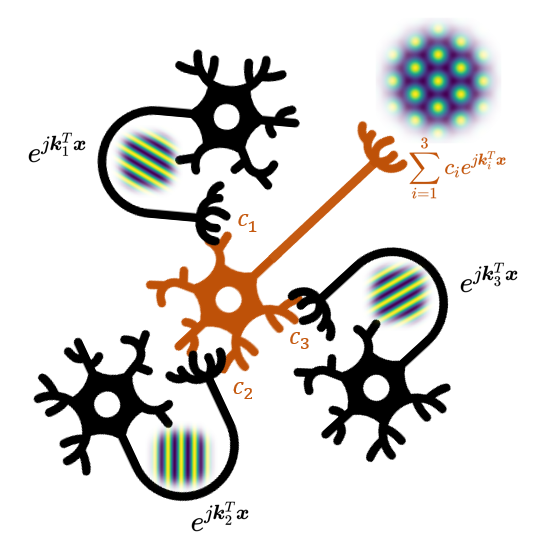
\includegraphics[width=0.9\columnwidth]{figures/Fig1.png}
\caption{Illustration of VCO theory. The black neurons are presynaptic neurons with simple oscillation in their dendrites. The orange neuron is the grid cell, whose grid firing pattern results from the summation of the three oscillation with different preferred direction.}
\label{fig1}
\end{figure}

\section{Derivation of Grid Cell Positional Encoding}
\subsection{Inner Product Translational Invariance}
Grid cells are not only responsible for representing absolute locations in Euclidean space but are also expected to encode relative spatial shifts between locations. This allows for the representation of free vectors from any starting location within the space, thereby facilitating vector-based navigation. The inner product of grid cell representations provides valuable insights into this capability. For a single grid cell, its representation at location \(\boldsymbol{x}\) is given by:

\begin{equation}
g(\boldsymbol{x}) = \sum_{i=0}^{n} c_i e^{j \boldsymbol{k}_i^T \boldsymbol{x}}
\end{equation}

Assume that \(\boldsymbol{x}\) deviates from \(\boldsymbol{y}\) by a fixed vector \(\boldsymbol{d}\) (i.e., \(\boldsymbol{x} - \boldsymbol{y} = \boldsymbol{d}\)). We then compute the functional inner product of \(g(\boldsymbol{x})\) with itself over the Euclidean space, that is. 

\begin{equation}
\begin{aligned} 
\left\langle g(\boldsymbol{x}), g(\boldsymbol{y}) \right\rangle _\mathcal{H} 
&= \int_{\mathcal{X}} \sum_{i=0}^{n} \sum_{m=0}^{n} c_i c_m^* e^{j(\boldsymbol{k}_i - \boldsymbol{k}_m)^T \boldsymbol{x}} e^{j \boldsymbol{k}_m^T (\boldsymbol{x} - \boldsymbol{y})} \\
&= \sum_{i=0}^{n} |c_i|^2 e^{j \boldsymbol{k}_i^T \boldsymbol{d}}
\end{aligned}
\end{equation}

That means for a given grid cell, the inner product of its activation map and its shifted version can represent the shift vector without consideration of any certain locations. Apparently, the inner product form a tranlational invariant kernel function $\kappa_0(\boldsymbol{x}, \boldsymbol{y})= \left \langle g(\boldsymbol{x})  , g(\boldsymbol{y}) \right \rangle _\mathcal{H} =h(\boldsymbol{x}- \boldsymbol{y})$. There are countless grid cells in the mammal's brain. The collective representation to the offset vector $\boldsymbol{d}$ can be expressed as follow as the summation of grid cell inner products:

\begin{equation}
\begin{aligned}
\sum_{g \in \mathcal{G}} \left\langle g(\boldsymbol{x}), g(\boldsymbol{y}) \right\rangle _\mathcal{H} 
&= \sum_{i} |c_i|^2 e^{j \boldsymbol{k}_i^T \boldsymbol{d}} \\
&\propto \int_{\mathbb{R}^2} p(\boldsymbol{k}) |c(\boldsymbol{k})|^2 e^{j \boldsymbol{k}^T \boldsymbol{d}} \, d\boldsymbol{k}
\end{aligned}
\end{equation}

Note this function is also a translational invariant kernel for $\boldsymbol{x}$ and $\boldsymbol{y}$. Simultaneuously, in its form it scale to the inverse Fourier transformation of the probability distribution of wave vectors. According to \emph{Bochner theorem} \cite{bochner2005harmonic}, we know this kernel, as the inverse Fourier transformation of a non-nagative measurement, is positive definite. Therefore, we can apply random Fourier feature (RFF) \cite{rahimi2007random} technique on this shift-invariant kernel, which demands positive definite kernel as the prerequisite. We denote the $\kappa(\boldsymbol{x}, \boldsymbol{y})$ as this kernel and we can know:

\begin{equation}
\begin{aligned}
\kappa(\boldsymbol{x}, \boldsymbol{y}) 
&= \int_{\mathbb{R}^2} p(\boldsymbol{k}) |c(\boldsymbol{k})|^2 e^{j \boldsymbol{k}^T \boldsymbol{d}} \, d\boldsymbol{k} \\
&= \mathbb{E}_{\boldsymbol{k}} \left[ |c(\boldsymbol{k})|^2 e^{j \boldsymbol{k}^T \boldsymbol{d}} \right] \\
&\approx \frac{1}{D} \sum_{i=1}^{D} \left( |c_i|^2 e^{j \boldsymbol{k}_i^T \boldsymbol{x}} \cdot e^{-j \boldsymbol{k}_i^T \boldsymbol{y}} \right) \\
&= \frac{1}{\sqrt{D}} 
\left( \begin{array}{c}
e^{j \boldsymbol{k}_1^T \boldsymbol{x}} \\
e^{j \boldsymbol{k}_2^T \boldsymbol{x}} \\
\vdots \\
e^{j \boldsymbol{k}_D^T \boldsymbol{x}}
\end{array} \right)^T \\
&\quad \cdot
\begin{bmatrix}
|c_1|^2 & & & \\
& |c_2|^2 & & \\
& & \ddots & \\
& & & |c_D|^2
\end{bmatrix} \\
&\quad \cdot
\left( \begin{array}{c}
e^{-j \boldsymbol{k}_1^T \boldsymbol{y}} \\
e^{-j \boldsymbol{k}_2^T \boldsymbol{y}} \\
\vdots \\
e^{-j \boldsymbol{k}_D^T \boldsymbol{y}}
\end{array} \right)
\frac{1}{\sqrt{D}}
\end{aligned}
\end{equation}

When considering the population activity of grid cells, we can disregard the constant \(\frac{1}{\sqrt{D}}\) that represents the population size. In this context, grid cells can be seen as the product of diagonalized input weights and a vector whose entries are Fourier bases with preferred directional preferences. This is analogous to Fourier analysis, where a function is decomposed into orthogonal bases and their corresponding coefficients. Consequently, the inner product of spatial-domain representation functions in the functional space is replaced by the inner product of frequency-domain vectors in a finite-dimensional vector space.

We propose that the brain represents Euclidean space using multi-dimensional Fourier analysis, akin to the auditory system's processing of sound waves and the visual system's processing of light waves. By integrating oscillations of various spatial frequencies, the grid cell encoding system can efficiently represent spatial information with high resolution. Furthermore, the Random Fourier Features (RFF) approach imposes no constraints on the dimensionality of locations \(\boldsymbol{x}\) and \(\boldsymbol{y}\). This suggests that the Fourier representation of grid cells can encode location information in arbitrarily high-dimensional spaces.

\subsection{Optimal Ratio of Grid Scale under Economy Principle}

In the derivation above, we assumed the wave vector (i.e., the preferred direction) follows a probability distribution, such as the uniform distribution often used in RFF. However, neuroscience evidence shows that the medial entorhinal cortex consists of several modules. Within the same module, the direction and period scale of the cell grids remain consistent, but these discretized scales shrink along the ventral-dorsal axis \cite{stensola2012entorhinal}, representing a transition from coarse, low-frequency to granular, high-frequency spatial information. The periodic ratio of the adjacent scale remains around 1.5, as estimated by both animal measurements and computational simulations \cite{stensola2012entorhinal, banino2018vector}. This hierarchical spatial representation demands significantly fewer grid cells while maintaining fine spatial resolution, or say the economy principle \cite{wei2015principle}.

The challenge now is to determine the optimal ratio of the grid scale, which is crucial for constructing a positional encoding system. Recall that in the original positional encoding of the Transformer architecture \cite{vaswani2017attention}, the encoding spatial frequency is calculated as \(\omega_k = \frac{1}{10000^{2k/d}}\), forming a geometric series of wavelengths. The rationale behind this choice remains unclear, and we anticipate that computational theories of grid cells can provide insights into frequency determination.

\begin{figure}
    \centering
    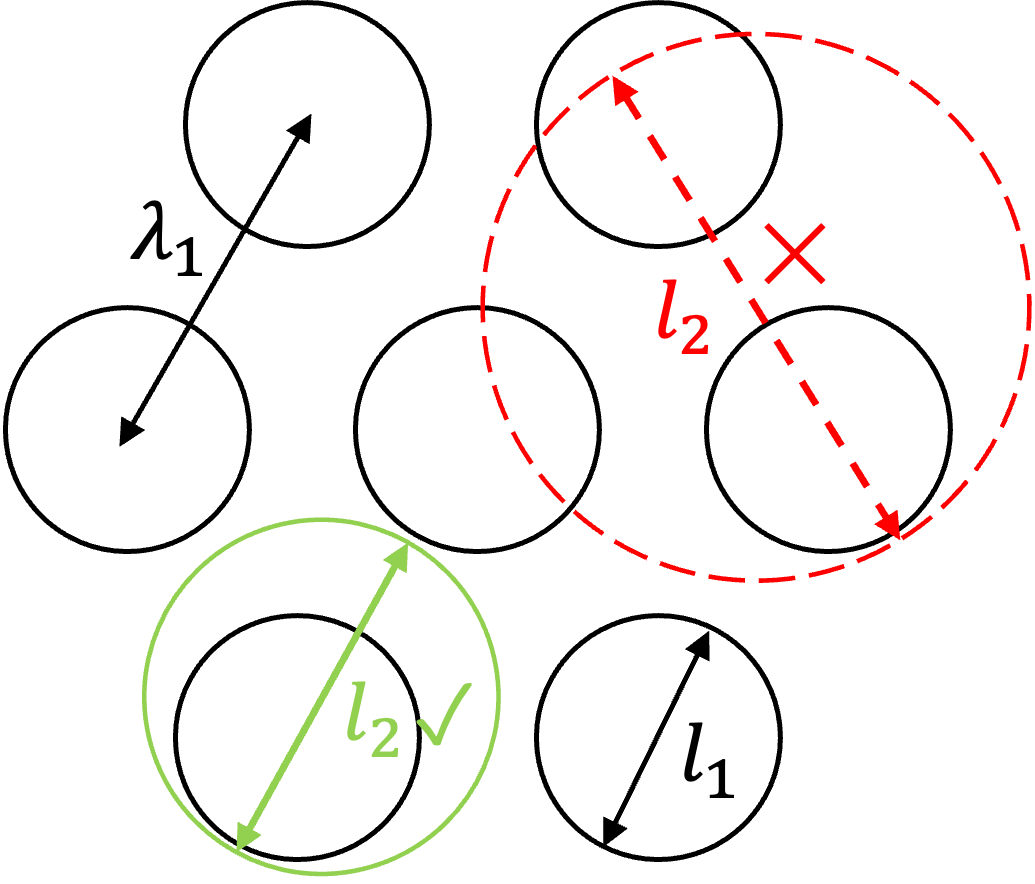
\includegraphics[width=0.9\columnwidth]{figures/Fig2.png}
    \caption{Illastration of relationship between firing fields diameter and periodicity. For two grid cells with adjacent discrete scale, the periodcity of the smaller scale must be less than the diameter of the larger one, otherwise the system cannot distinguish two locations.}
\end{figure}

Here we provide a generalized derivation based on the proof in \cite{wei2015principle}. We aim to represent \emph{p}-dimensional Euclidean space with the least number of grid cells, reflecting the principle of economy. Assume there are \(m\) scales (or layers) of the grid cells. The period of the \(i\)-th module layer (\(i=1,2,\ldots,m\)), or the distance between the adjacent grid vertices, is denoted as \(\lambda_i\). The period increase as $i$ becomes larger. The scale ratio of the adjacent layers is \(r = \lambda_{i+1}/\lambda_{i} > 1\). A grid field is a hyperspherical area centered around a grid vertex in the space, with its diameter denoted as \(l_i\). For 2D space, a grid field is a circular-plate area activating the grid cell. Clearly, to cover the whole space without omissions, more than one grid cell with different phases are required. The larger the ratio of \(\lambda_i\) to \(l_i\), the more grid cells are needed. If there must be at least \(d\) cells responding to a spatial location, the total number of grid cells across all layers can be expressed as $N$:

\begin{equation}
    N = \sum_{i=1}^{m} d \left( \frac{\lambda_i}{l_i} \right)^p
\end{equation}

Apart from that, the condition $l_{i} \le \lambda_{i-1}$ must be satisfied. If not, the grid cell system cannot ascertain current location when cells from both layer $i$ and $i+1$ fire simultaneously, because the larger firing field contains more than one smaller fields, as shown in Figure 2. The condition derives $l_{i} \le \lambda_{i} / r$. If the grid cell system must represent the space at a given constant spatial resolution $R$, that is, we predefined the measurement relationship between the largest scale and the smallest firing field unit:

\begin{equation}
R = \left(\frac{\lambda_m}{l_1}\right)^p 
  = \left(\prod_{i=0}^{m-1} \frac{\lambda_{i+1}}{\lambda_i}\right)^p 
  = \left(r^p\right)^m
\end{equation}

Here we set the $\lambda_0 = l_1$. When we denote $r^p = \rho$ we get:

\begin{equation}
N = d \sum_{i=1}^{m} \left( \frac{\lambda_i}{l_i} \right)^p \ge dmr^p 
  = d \rho \log_\rho R
\end{equation}

By differentiation, we find that when \(\rho = e\), which means \(r = \sqrt[p]{e}\), we achieve the minimal number of grid cells, adhering to the principle of economy. In summary, a hierarchical grid cell representation can, with a limited population number, efficiently cover the space. The theoretically optimal scale ratio for \(p\)-dimensional space is \(r = \sqrt[p]{e}\).

In the original Transformer architecture, the adjacent scale of positional encoding is described by Equation \ref{eq_ratio}. For instance, when the encoding dimension \(d_{\text{model}}\) is 128, the difference in adjacent scales is \(10000^{\frac{2}{128}} \approx 1.457\), whereas for an encoding dimension of 512, the difference in adjacent scales is \(10000^{\frac{2}{512}} \approx 1.036\). This relationship can be expressed as follows:

\begin{equation}
\label{eq_ratio}
\rho_{\text{ratio}} = \frac{10000^{\frac{2(i+1)}{d_{\text{model}}}}}{10000^{\frac{2i}{d_{\text{model}}}}} = 10000^{\frac{2}{d_{\text{model}}}}
\end{equation}

As discussed, to avoid ambiguity in positional encoding, the maximum scale ratio for encoding in an \(n\)-dimensional space is \(r = \sqrt[p]{e}\). Consequently, the minimum encoding dimension can be determined when the base is 10000. To achieve an adjacent scale difference of \( \sqrt[p]{e} \), we can establish the following inequality:

\begin{equation}
10000^{\frac{2}{d_{\text{model}}}} \leq \sqrt[p]{e}
\end{equation}

Taking the logarithm of both sides and solving for \(d_{\text{model}}\):

\begin{equation}
\frac{2}{d_{\text{model}}} \log(10000) \leq \frac{1}{p} \log(e)
\end{equation}

\begin{equation}
d_{\text{model}} \geq \frac{2 \log(10000) p}{\log(e)}
\end{equation}

This allows us to calculate the minimum encoding dimension \(d_{\text{model}}\) that satisfies the specified adjacent scale difference.


\subsection{Proposal of Grid-cell Positional Encoding (GridPE)}

After demonstrating the capability of representing relative movement in space through inner product calculations and determining the optimal ratio of encoding periods, we introduce a unified positional encoding scheme for attention-based architectures. Inspired by neuroscientific principles of grid cells, our method extends the foundational ideas presented by \cite{su2024roformer}. While Su’s model combines absolute and relative positional encodings within a fixed framework, our schema advances this by incorporating grid cell-inspired encodings that inherently support extrapolation to higher dimensions and maintain translational invariance. Notably, in one-dimensional space, where GridPE can be expressed using a single Fourier basis, our encoding scheme is equivalent to rotational positional encoding. This demonstrates the flexibility of our approach and its alignment with established encoding strategies, further enhancing its applicability across various architectural contexts. According to Su's model, to accommodate both absolute and relative positional encoding, the inner product of the query $\boldsymbol{q}$ and key $\boldsymbol{k}$, which represents their similarity, can be modified as follows:

\begin{equation}
\left\langle \boldsymbol{q}', \boldsymbol{k}' \right\rangle = \boldsymbol{q}^T \boldsymbol{W}_m^T \boldsymbol{W}_n \boldsymbol{k}
\end{equation}

Here $m$ and $n$ refer to the position of the query and key respectively. The multiplication of $\boldsymbol{W_m}$ and $\boldsymbol{W_n}$ is the function of the relative position $m-n$. We can encode the position $m$ based on the grid cell encoding rationale. Assume there are $d$ dimensions for the embedded queries and keys, we also set $d$ layers of different scale of grid cell. Then we can set the positional code as below: 

\begin{equation}
\label{eq13}
\boldsymbol{W}_m = \left[
\begin{array}{c}
\sum_{i} c_{i} e^{j \boldsymbol{\omega}_{i,1}^T m} \\
\sum_{i} c_{i} e^{j \boldsymbol{\omega}_{i,2}^T m} \\
\vdots \\
\sum_{i} c_{i} e^{j \boldsymbol{\omega}_{i,d}^T m}
\end{array}
\right]
\end{equation}

Here we substitute the symbol of the wave vector $\boldsymbol{k}$ with $\boldsymbol{\omega}$ in case of confusion of key. We can see the inner product of the two positional codes $\boldsymbol{W}_m^T\boldsymbol{W}_n$ preserve the translational invariance. To fulfill the positional encoding in the neural network, we proposed several strategies as the variants to integrate the position information into the queries or keys.

\paragraph{Representing Encodings as Rotation Matrices} If the information to be encoded (query or key) is a \(d\)-dimensional vector, and \(d\) is even, then the positional codes can be calculated as follows:

\begin{equation}
\boldsymbol{R}_m = 
\begin{bmatrix}
    \boldsymbol{A}_1 & \boldsymbol{0} & \dots & \boldsymbol{0} \\
    \boldsymbol{0} & \boldsymbol{A}_2 & \dots & \boldsymbol{0} \\
    \vdots & \vdots & \ddots & \vdots \\
    \boldsymbol{0} & \boldsymbol{0} & \dots & \boldsymbol{A}_{d/2} \\
\end{bmatrix}
\end{equation}
    
\begin{equation}
\boldsymbol{A}_k = 
\begin{bmatrix}
    \Re\left(e^{j \boldsymbol{\omega}_{k,1}^T m}\right) & -\Im\left(e^{j \boldsymbol{\omega}_{k,1}^T m}\right) \\
    \Im\left(e^{j \boldsymbol{\omega}_{k,1}^T m}\right) & \Re\left(e^{j \boldsymbol{\omega}_{k,1}^T m}\right) \\
\end{bmatrix}
\end{equation}

\begin{equation}
\left\langle \boldsymbol{q}', \boldsymbol{k}' \right\rangle = \boldsymbol{q}^T \boldsymbol{R}_m^T \boldsymbol{R}_n \boldsymbol{k}
\end{equation}
    
The $\Re(\cdot)$ and $\Im(\cdot)$ respectively means the extraction of the real and imagery part. The purpose of this strategy is to encode the position by constructing the rotation matrix. The rotation angles comes from the grid cell Fourier functions. 

\paragraph{Incorporating Real and Imaginary Parts into Information Vectors} We can also extract the real and imagery part and add them into the information vectors, similar to the original Transformer architecture:

\begin{equation}
\boldsymbol{q}' = \Re\left(\boldsymbol{W}_m\right) + \Im\left(\boldsymbol{W}_m\right) + \boldsymbol{q}
\end{equation}

After the encoding, the similarity of encoded queries and key can be calculated as vector dot product.

\paragraph{Preserving the Complex Form} We can directly use the real part of the inner product between two sets of "complex" position encoding as the encoding product.

\begin{equation}
\left\langle \boldsymbol{q}', \boldsymbol{k}' \right\rangle = \boldsymbol{q}^T \Re\left(\boldsymbol{W}_m^H \boldsymbol{W}_n\right) \boldsymbol{k}
\end{equation}

The Hermite operator means the conjugate transpose of the complex matrix.

\paragraph{Feature Mapping of Positional Encoding Using Deep Learning} Finally, we can transform the original positional encoding by applying a trained deep neural network.

\begin{equation}
\left\langle \boldsymbol{q}', \boldsymbol{k}' \right\rangle = \boldsymbol{q}^T f_\theta(\boldsymbol{W}_m^T) f_\theta(\boldsymbol{W}_n) \boldsymbol{k}
\end{equation}

where $f_\theta(\cdot)$ is a neural network projection (e.g. a multi-layer perceptrons) parameterized by $\theta$. The projection does not change the dimension of the encoding.

\section{Experiments}
\subsection{Property of Distance Decay}

We first display that our positional encoding approach exhibits the property of distance decay in any high-dimensional space. This implies that the association between two positions diminishes as the distance between them increases. We select a square area in two-dimensional space, calculating the positional encoding vector within the area as shown in Equation \ref{eq13}, and compute the inner products between the central "core" point and uniformly sampled points. Given that we have proven the translational invariance of the inner product, our findings remain valid when any other point is chosen as the core. Figure \ref{fig3} presents the inner product surface plot and a profile plot with \(x\) fixed at \(0.5\).

% \begin{figure}[htbp]
% \centering
% 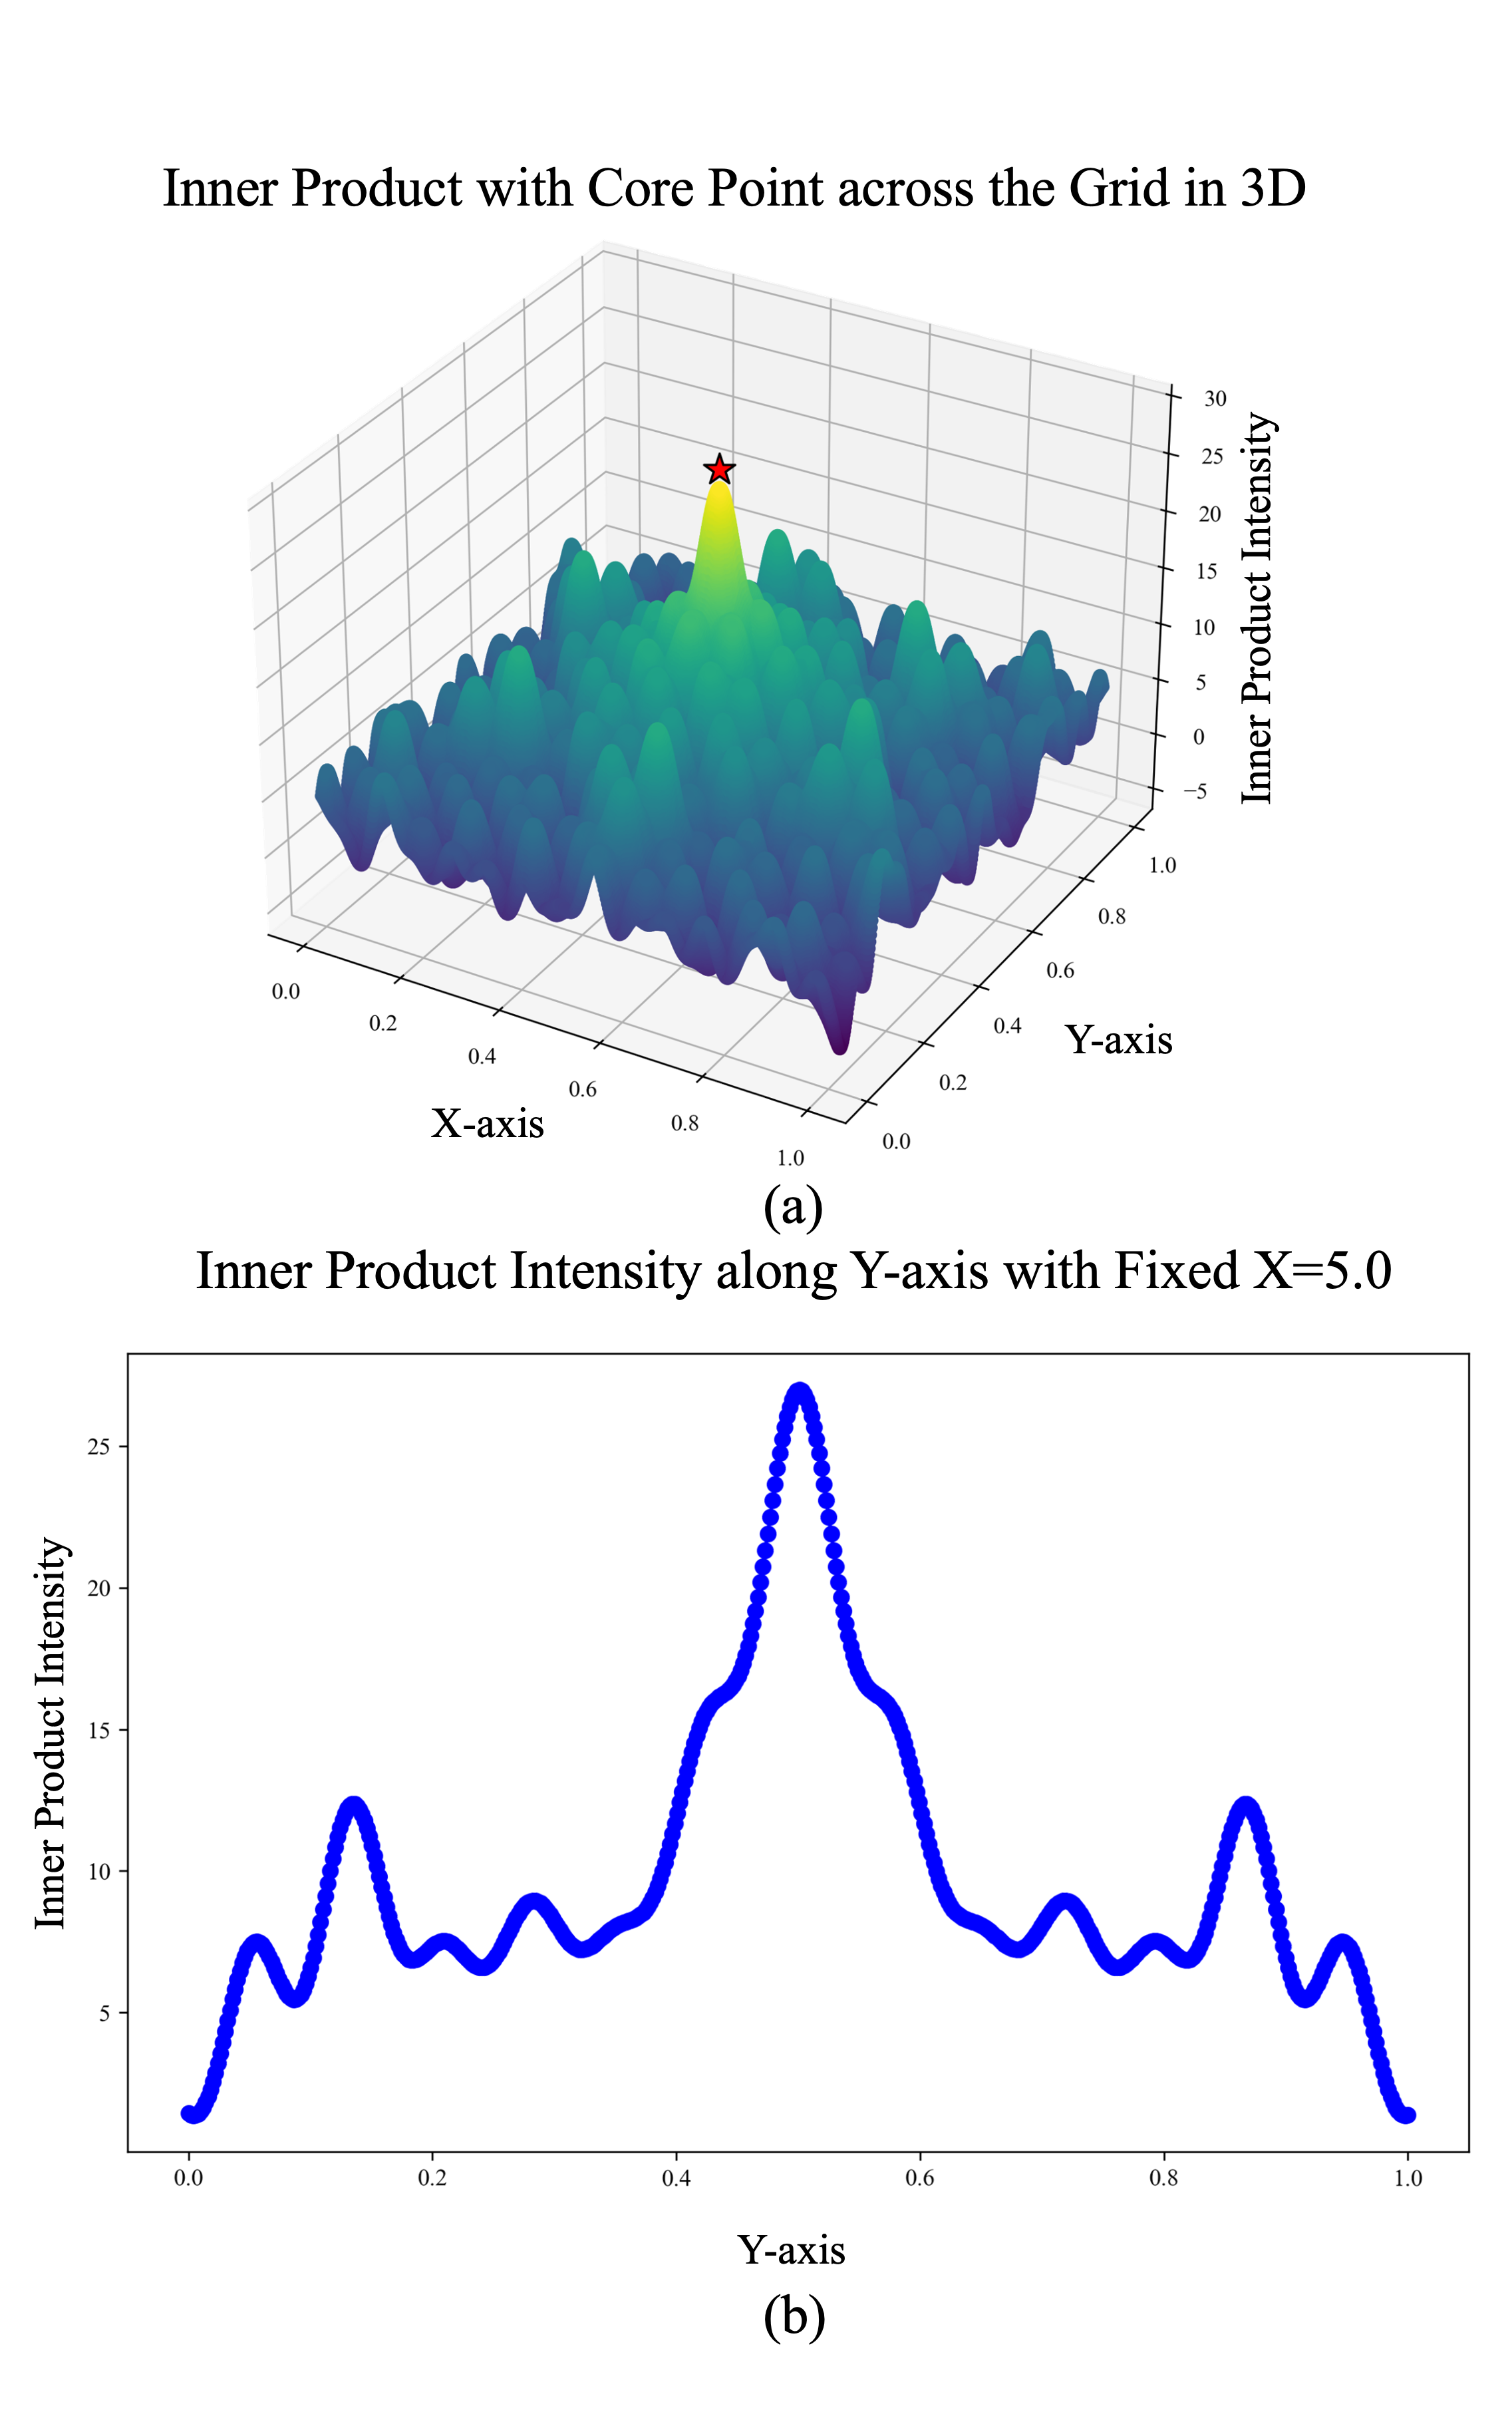
\includegraphics[width=0.9\columnwidth]{figures/Fig3.png}
% \caption{The inner products intensity with the core points $(0.5, 0.5)$ of points in the unit square area. Left: the distribution of inner products is shown as a surface plot across the area. Right: a profile plot showing the inner products between core points and points with fixed $x=0.5$.}
% \label{fig3}
% \end{figure}

We observe that the inner product exhibits an overall decreasing trend as the spatial distance increases, with points near the core having relatively larger inner products. Despite this, local sinusoidal fluctuations, resulting from the Fourier function form, are still evident. These calculations corroborate the effectiveness of our encoding method in representing spatial distance relationships.

\begin{figure}[t]
    \centering
    \begin{subfigure}[b]{0.8\columnwidth}
        \centering
        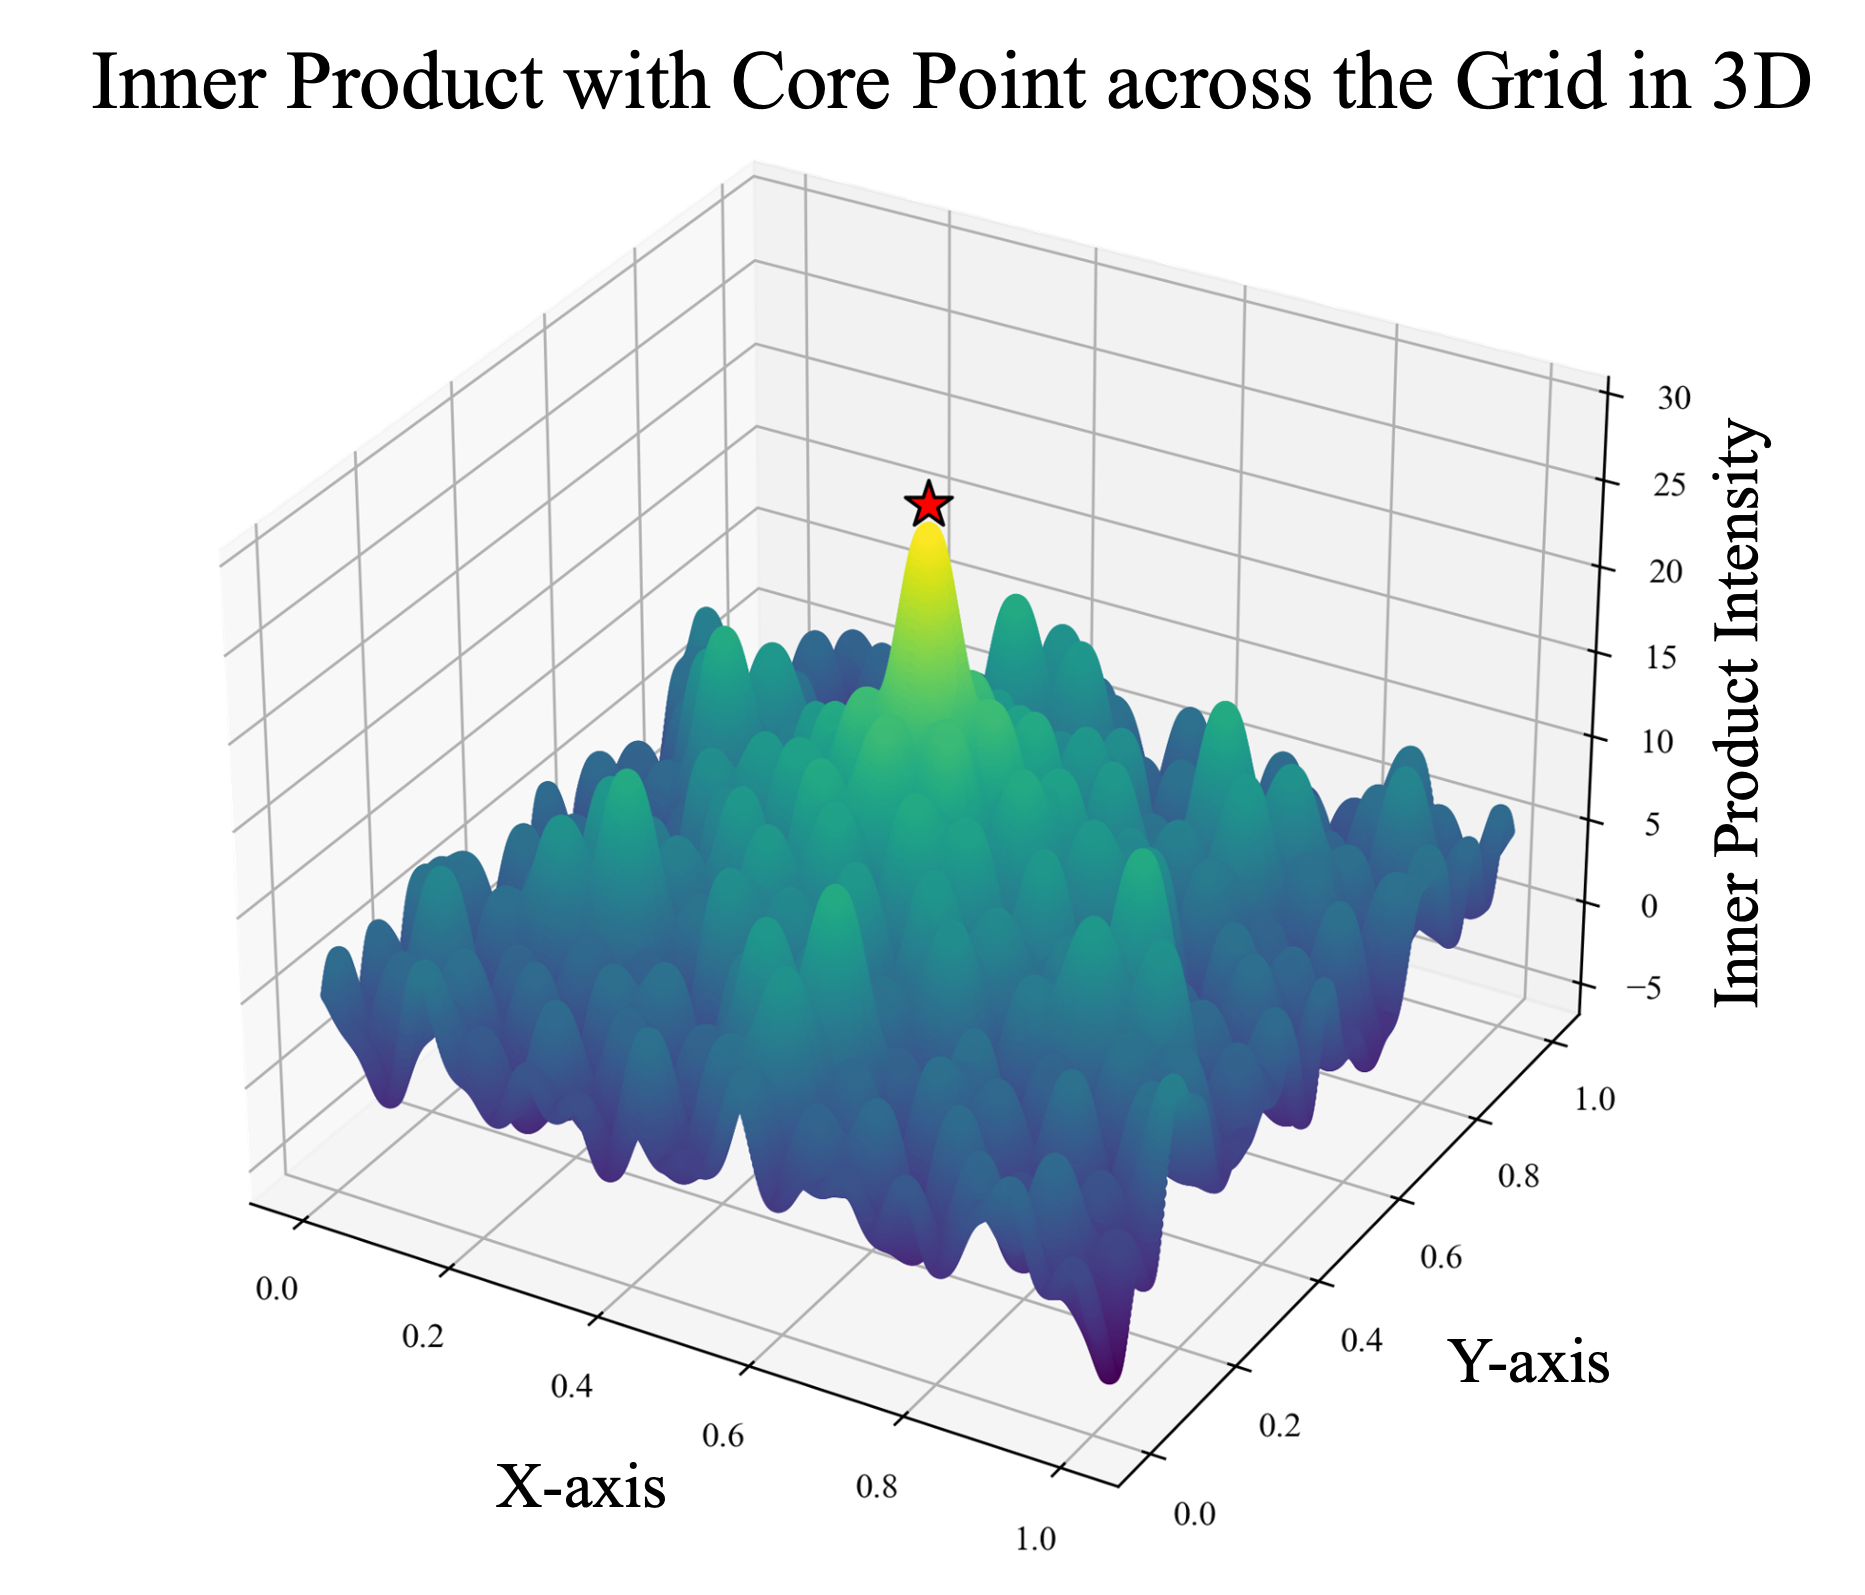
\includegraphics[width=\textwidth]{figures/Fig3_1.png}
        % \caption{Inner Product with Core Point in 3D}
        % \label{fig:fig3_3d}
    \end{subfigure}
    \vspace{10pt} % 可以调整间距
    \begin{subfigure}[b]{0.8\columnwidth}
        \centering
        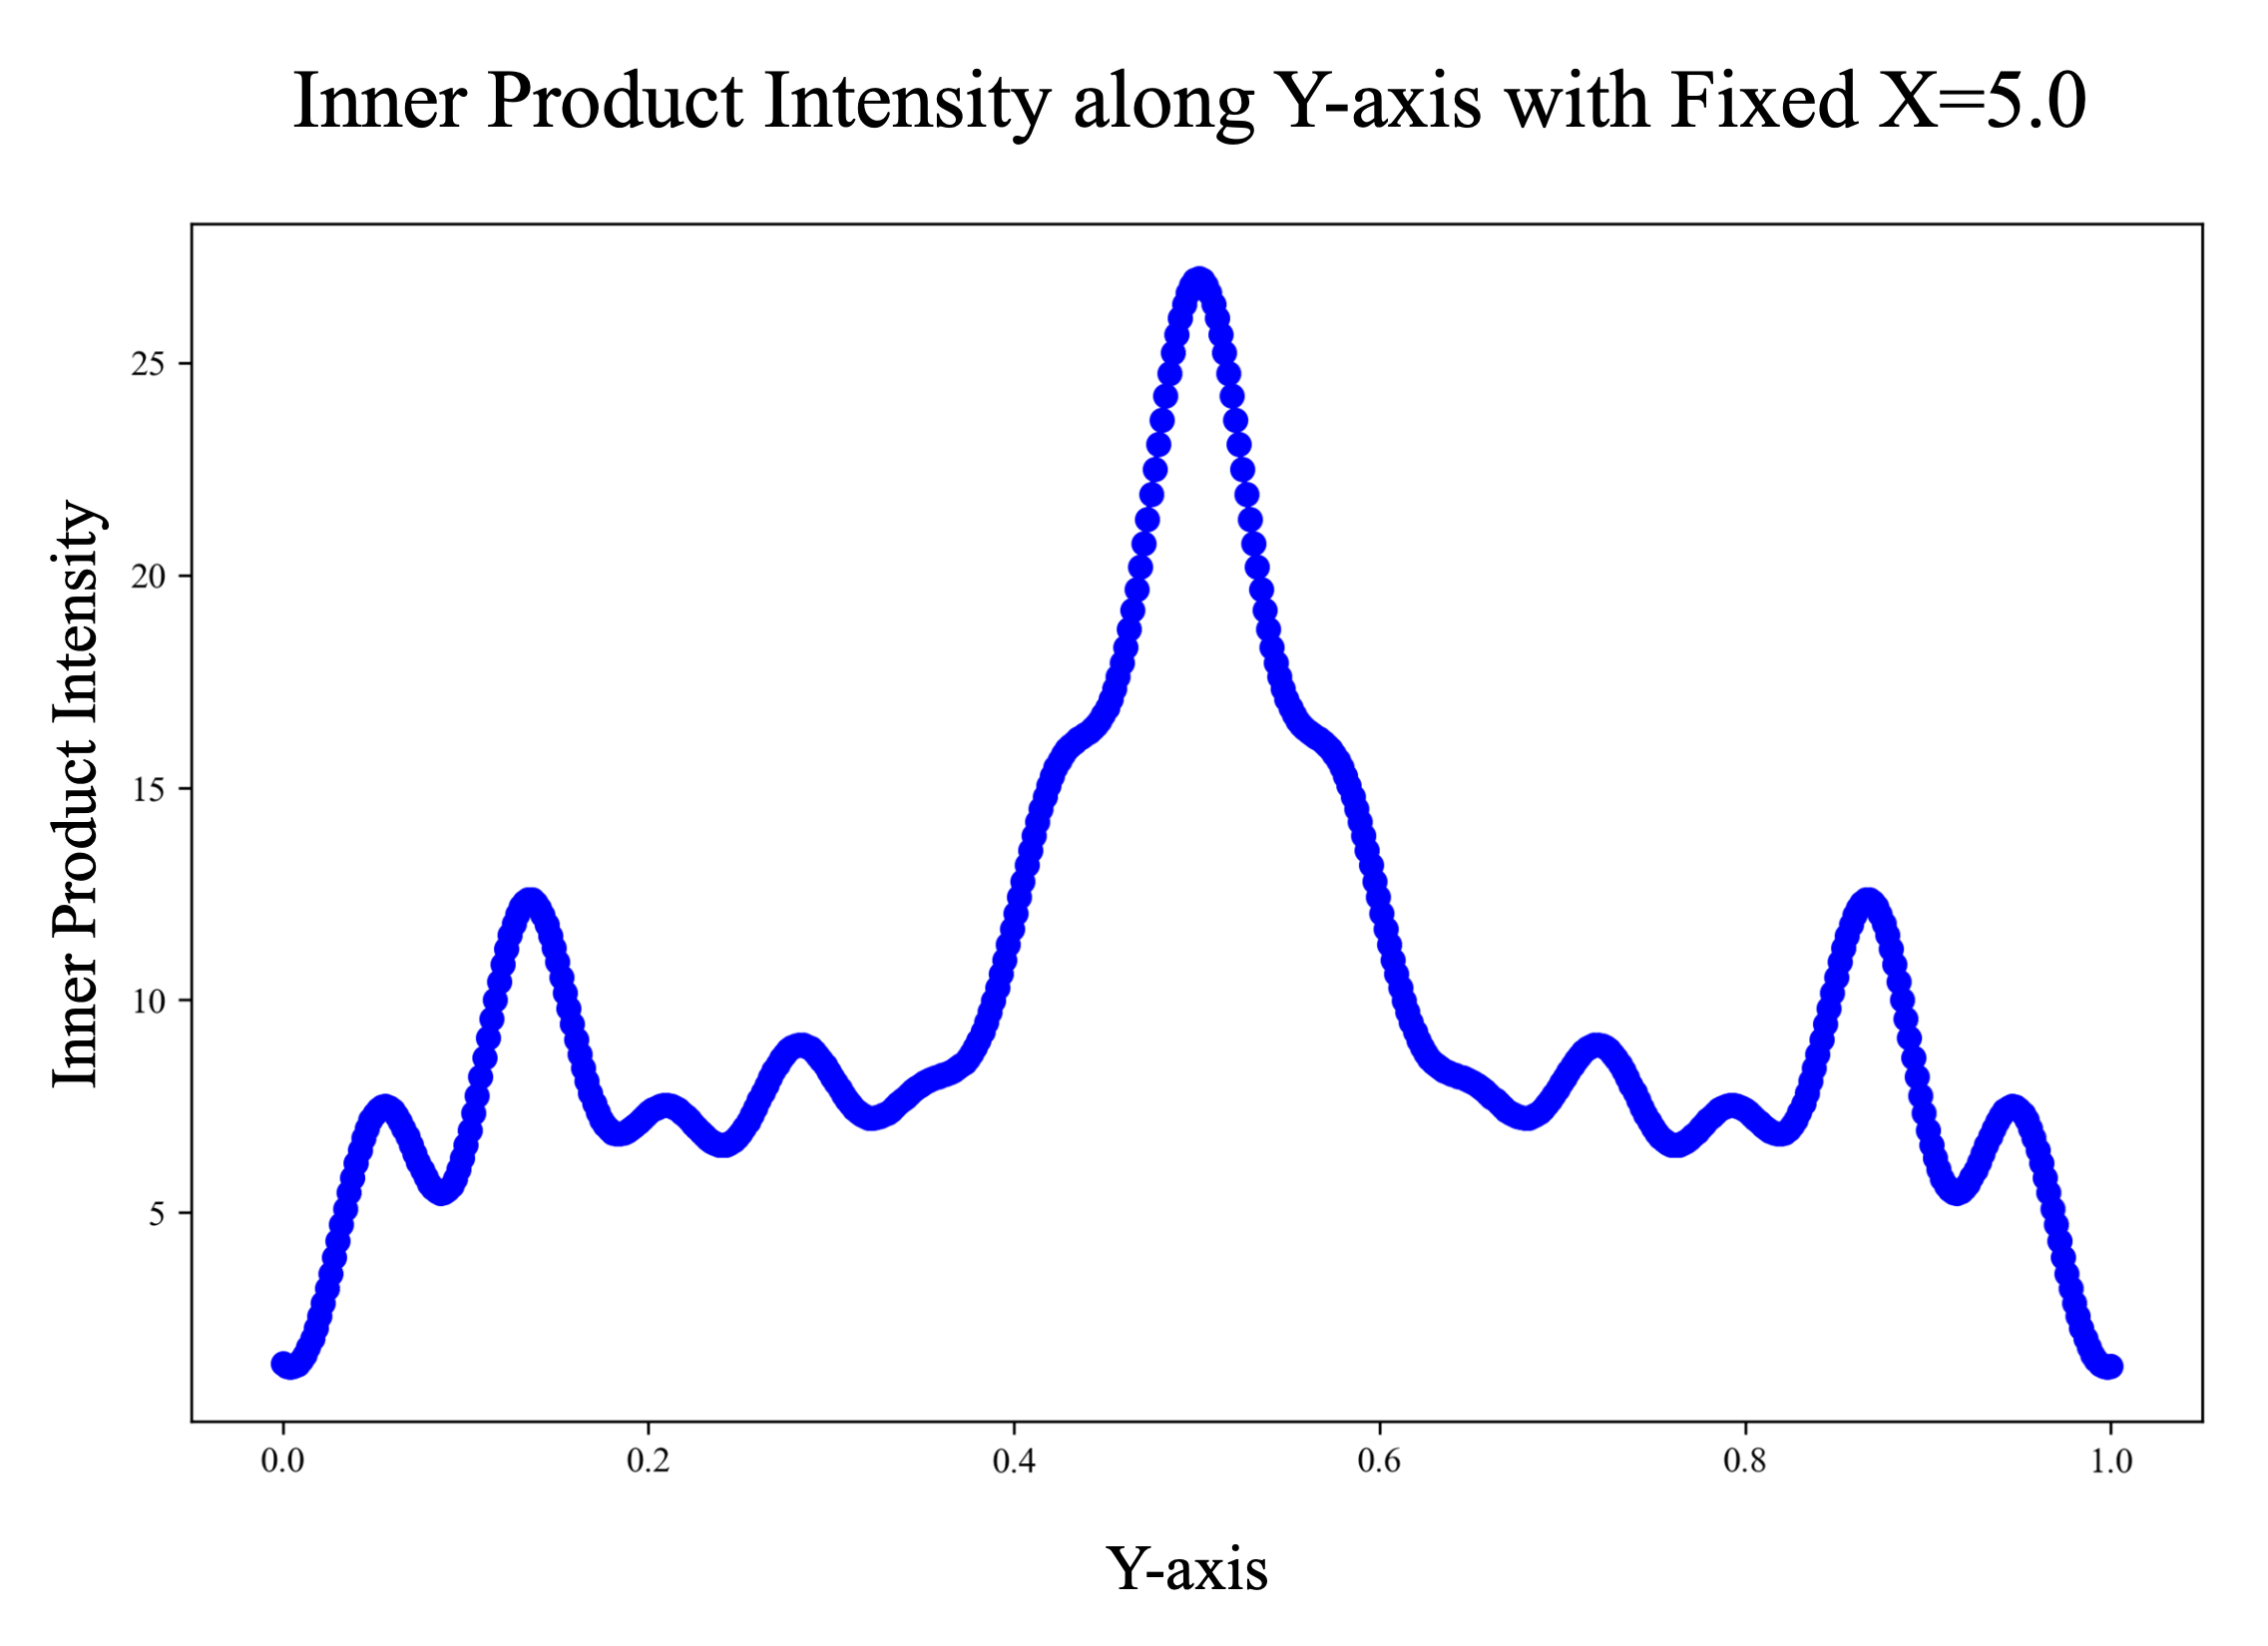
\includegraphics[width=\textwidth]{figures/Fig3_2.png}
        % \caption{Inner Product along Y-axis with Fixed X=0.5}
        % \label{fig:fig3_profile}
    \end{subfigure}
    \caption{The inner products intensity with the core points $(0.5, 0.5)$ of points in the unit square area. Left: the distribution of inner products is shown as a surface plot across the area. Right: a profile plot showing the inner products between core points and points with fixed $x=0.5$.}
    \label{fig3}
\end{figure}

\subsection{Performance of GridPE on Visual Task}

To empirically validate the capability of GridPE strategies in encoding positional information, we draw on previous research \cite{chu2021Twins, chu2023CPVT} and design an image classification task to evaluate neural network architectures with different positional encodings. We select the Pyramid Vision Transformer (PVT) \cite{wang2021pyramid} and Vision Transformer (ViT) \cite{dosovitskiy2020image} as the base architectures.

\subsubsection*{Baseline model descriptions.} 
PVT introduces a pyramid structure into the transformer architecture, which reduces input resolution and computational cost while enhancing performance in dense prediction tasks by effectively capturing multi-scale features. ViT, on the other hand, revolutionizes image classification by applying the transformer model to fixed-size image patches, leveraging global self-attention to model relationships across the entire image. 

\subsubsection*{Dataset.} 
We utilize the ImageNet-100 dataset, a subset of the widely recognized ImageNet dataset, to design our classification task. With its diverse and complex imagery, ImageNet-100 serves as an ideal benchmark for evaluating the effectiveness of GridPE in encoding positional information, rigorously testing the model's ability to handle high-dimensional and varied visual inputs. For our task, we partition 20\% of the images into a validation set, while the remaining 80\% are used for training, ensuring robust model evaluation and effective training during the experiment.

\subsubsection*{Implementation details.} 
We train the neural networks on a system with an NVIDIA RTX 4090 GPU using the PyTorch framework. Models are trained for 200 epochs with the AdamW optimizer and a batch size of 32. The `ReduceLROnPlateau` scheduler is employed to halve the learning rate if validation accuracy does not improve for 10 consecutive epochs, helping to fine-tune the model and prevent overfitting. PVT models use an image size of 384, while ViT models use 224. These settings ensure robust training and evaluation on the ImageNet-100 dataset.

\subsubsection{Results and Analysis}
We assess the effectiveness of GridPE by comparing models with different positional encoding strategies applied to two core attention-based architectures: PVT and ViT. For PVT, we evaluate the original version without explicit two-dimensional positional encoding (PVT-o), a variant using classical sinusoidal encoding (PVT-abs) \citep{vaswani2017attention}, and a model incorporating conditional positional encoding (CPVT) \citep{chu2023CPVT}. Additionally, we introduce four GridPE-enhanced versions—GridPVT-rotate, GridPVT-complex, GridPVT-deep, and GridPVT-merge—each reflecting different grid cell-inspired positional encoding strategies. We also apply these GridPE variants to the ViT architecture to examine their impact on a simpler and less parameter-intensive model. By comparing these GridPE-enhanced versions with the baseline ViT model, we aim to elucidate the influence of GridPE across models with varying architectural complexities.

\begin{table}[htb]
    \centering
    \resizebox{\columnwidth}{!}{%
    \begin{tabular}{@{}lccc@{}}
    \toprule
    Model Name         & Acc@1 (\%) & Acc@5 (\%) & Loss  \\ \midrule
    PVT-o              & 84.1       & 96.2       & 1.467 \\
    CPVT               & \textbf{87.1}    & 95.8        & 1.498 \\
    PVT-abs            & 85.3       & 96.6       & 1.483 \\
    GridPVT-rotate     & 82.3       & 95.7       & 1.511 \\
    GridPVT-complex       & 83.0       & 95.9       & 1.507 \\ 
    GridPVT-deep      & 84.6       & \textbf{97.4}        & \textbf{1.445} \\
    GridPVT-merge    & 82.9       & 95.8       & 1.514 \\  
    \midrule
    ViT                & 76.1       & 93.0       &  0.8234\\
    GridViT-rotate     & 77.6       & 91.5       & 0.9832 \\
    GridViT-complex    & 78.8       & 93.7       & 0.8691 \\
    GridViT-deep       & \textbf{81.5}       & \textbf{94.2}       & \textbf{0.4676} \\
    GridViT-merge      & 79.0       & 94.0       & 1.083 \\ \midrule
    \end{tabular}%
    }
    \caption{Comparative Analysis of Different Position Encoding Methods in Image Classification Tasks}
    \label{tab:model_performance}
\end{table}

% Table \ref{tab:model_performance} presents the comparative results. The outcomes of the PVT-based experiments indicate that the Grid Positional Encoding (GridPE) enhanced models do not outperform their counterparts, particularly the state-of-art model scale. It appears that the benefits of positional encoding may not be fully realized in such models, potentially due to smaller model scale with fewer parameters to capture complex spatial relationships. Nonetheless, an analysis of the training curves (as depicted in Figure \ref{fig:validation_pvt_accuracy}) reveals that the GridPE-enhanced models do not lag significantly behind in terms of training speed and validation accuracy. While the models may not achieve superior performance metrics, they maintain competitive training dynamics. Among the GridPE-enhanced models, the GridPVT-merge and GridPVT-complex variants achieve relatively better results. These models demonstrate higher prediction accuracy and exhibit smaller validation loss, indicating their potential to offer improved performance when scaled up or further optimized.

% For the ViT architecture, the application of GridPE variants also results in noticeable improvements across key metrics. GridViT-deep emerges as the standout model, achieving the highest top-1 accuracy at 81.5\%, top-5 accuracy at 94.2\%, and the lowest loss at 0.4676 among all evaluated ViT models. The improved performance of GridViT-deep, particularly its ability to attain both the highest accuracy and the lowest loss, highlights the versatility and strength of the GridPE method. This model’s success suggests that the depth and complexity of GridPE contribute significantly to the model’s learning capabilities, allowing it to generalize better on unseen data.

Table \ref{tab:model_performance} presents the comparative results, showing how different positional encoding strategies impact the performance of PVT and ViT models. Among these PVT models, CPVT achieves the highest top-1 accuracy (87.1\%), while GridPVT-deep excels with the best top-5 accuracy (97.4\%) and the lowest loss (1.445). The convergence curves in Figure \ref{fig:validation_pvt_accuracy} reveal that PVT models generally maintain stable and efficient convergence regardless of the positional encoding used, likely due to their complex architecture and larger parameter count. This complexity allows the PVT models to capture intricate spatial relationships, minimizing the impact of different positional encodings on their convergence speed and overall performance. 

For the ViT architecture, the application of GridPE variants results in noticeable improvements in performance, as seen in Table \ref{tab:model_performance}. GridViT-deep emerges as the most successful variant, achieving the highest top-1 accuracy (81.5\%) and the lowest loss (0.4676), representing significant gains over the baseline ViT model. The validation accuracy curves in Figure \ref{fig:validation_accuracy} highlight that ViT models, which are simpler and have fewer parameters compared to PVT models, are more sensitive to changes in positional encoding. While other variants such as GridViT-complex and GridViT-merge also outperform the baseline ViT model, they exhibit higher losses, suggesting that while GridPE can enhance accuracy, it may require further tuning to optimize efficiency and convergence. This underscores the importance of carefully matching positional encoding strategies with the model architecture to achieve the best performance outcomes.

\begin{figure}[htb]
    \centering
    \begin{subfigure}[b]{0.5\textwidth}
        \centering
        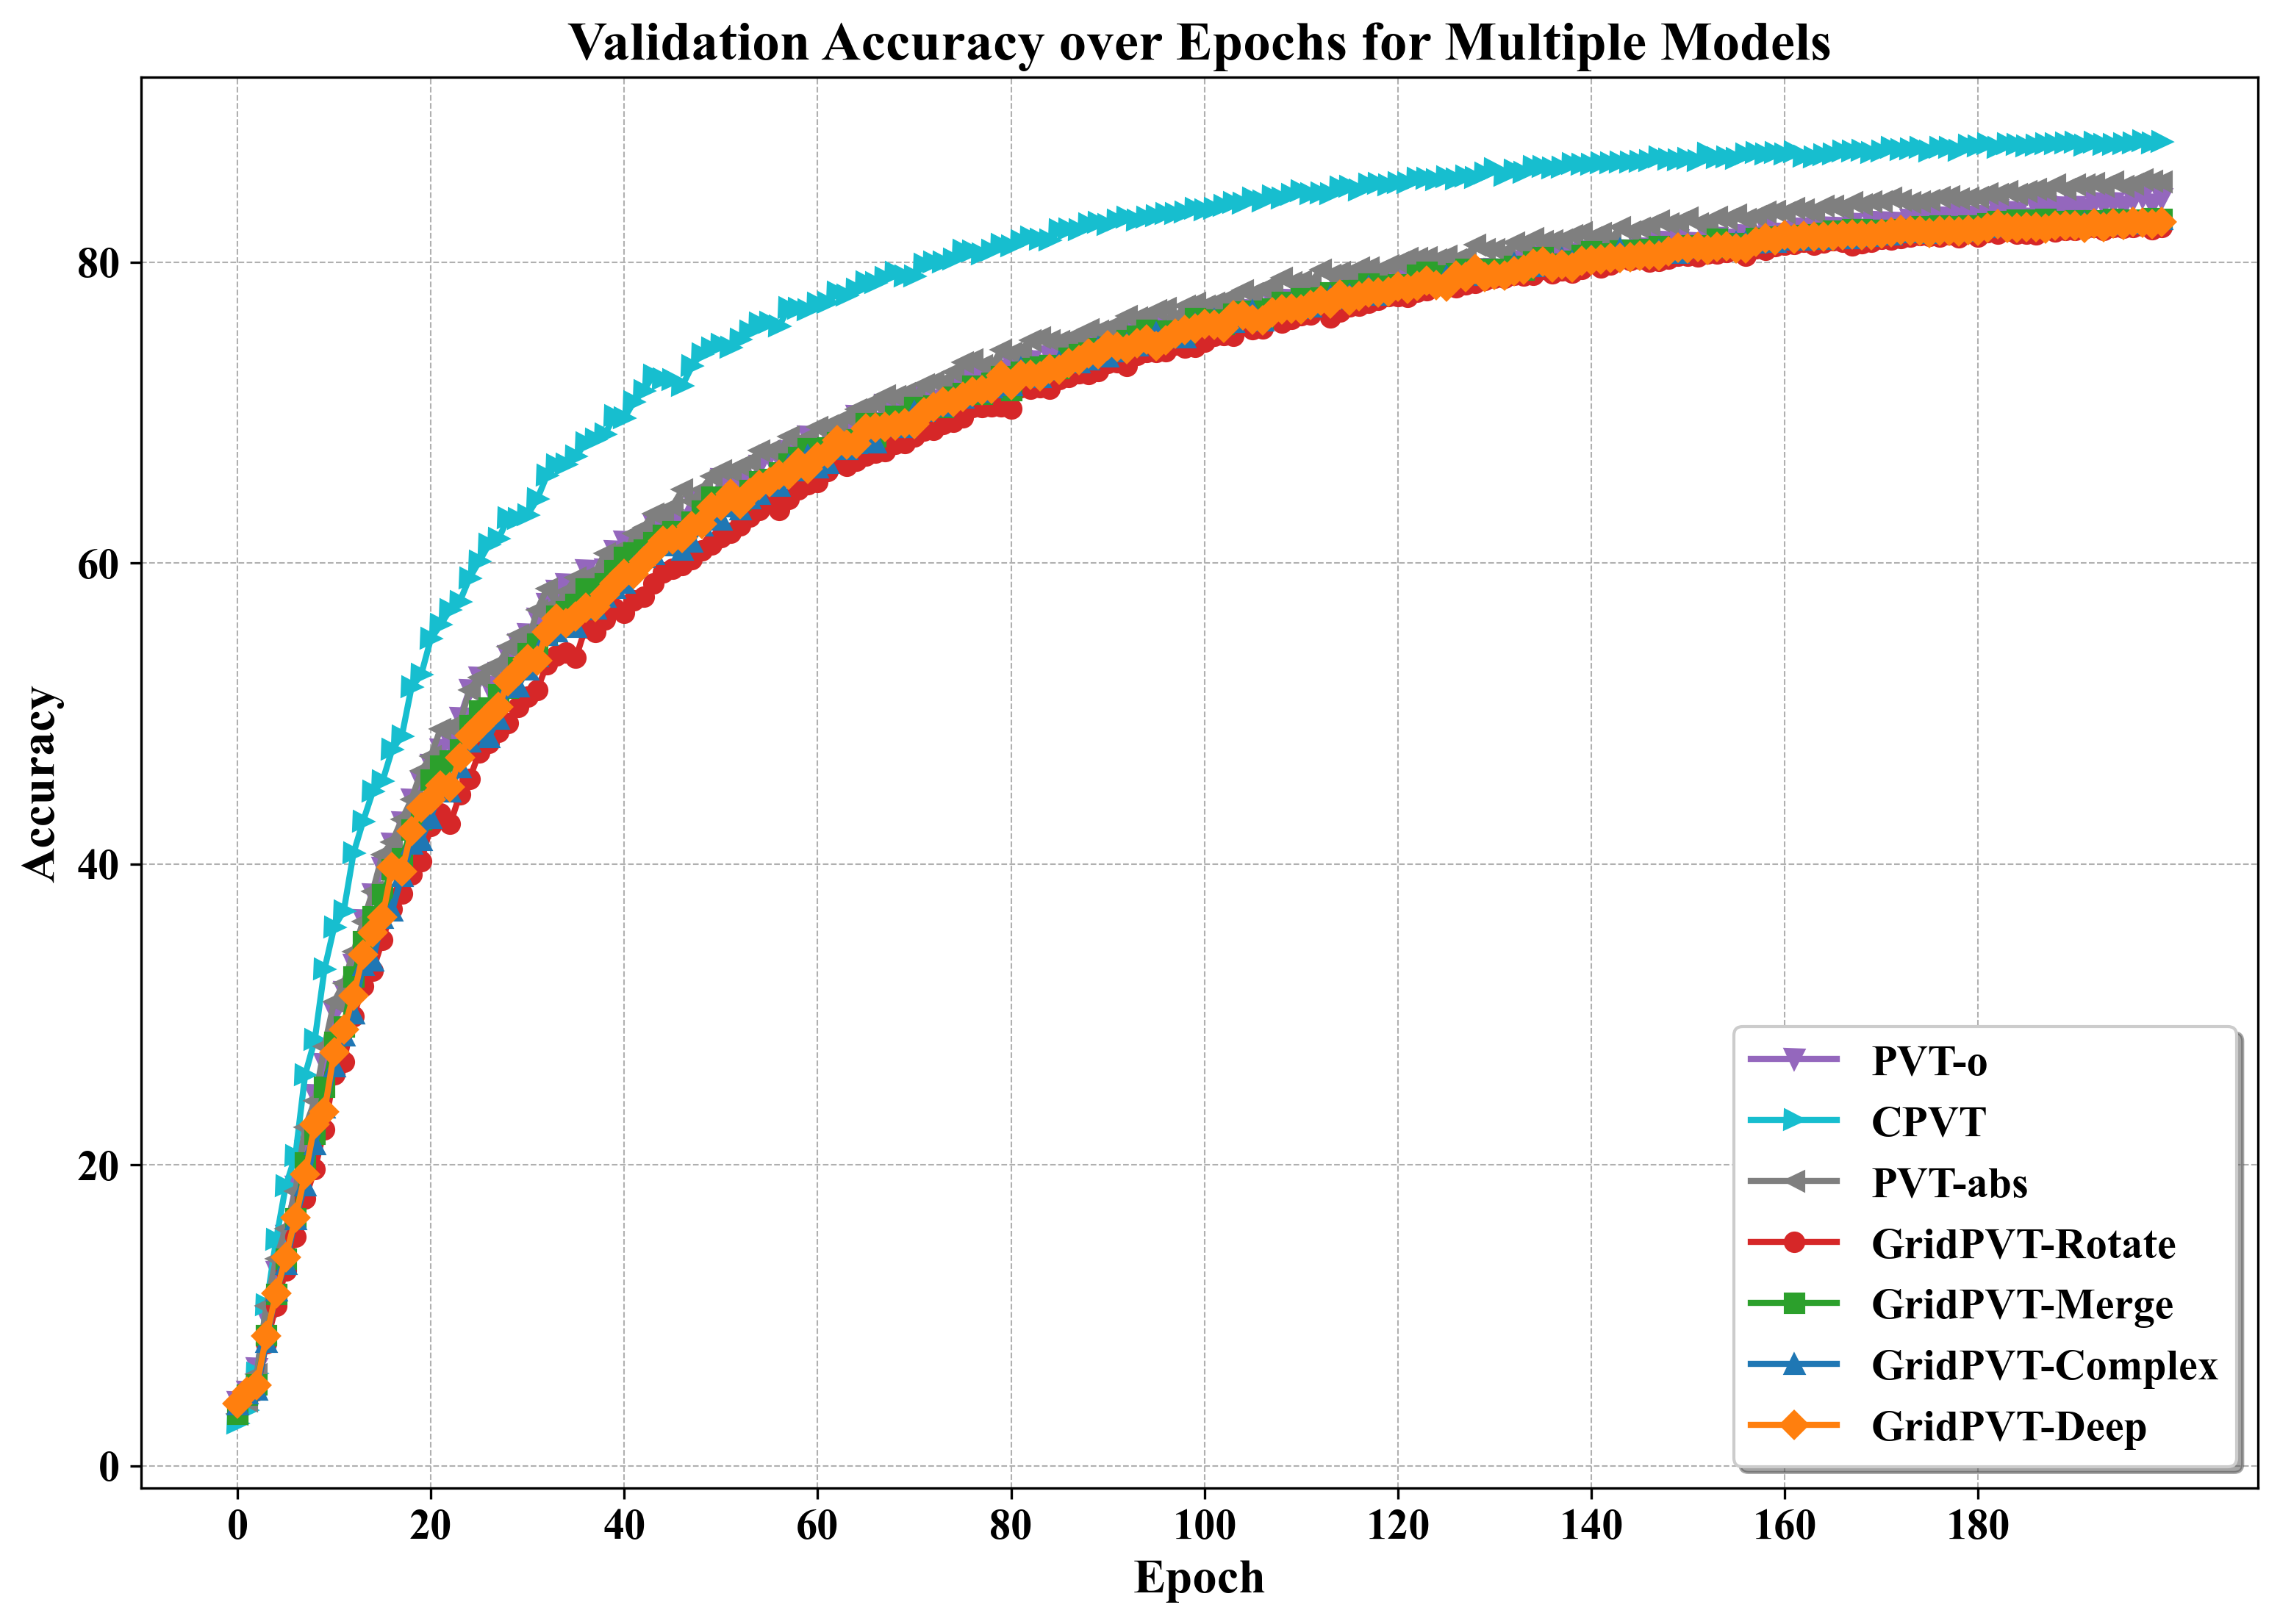
\includegraphics[width=\textwidth]{figures/Fig5.png}
        \caption{Validation Accuracy over Epochs for Multiple Variants of PVT Models.}
        \label{fig:validation_pvt_accuracy}
    \end{subfigure}
    \hfill
    \begin{subfigure}[b]{0.5\textwidth}
        \centering
        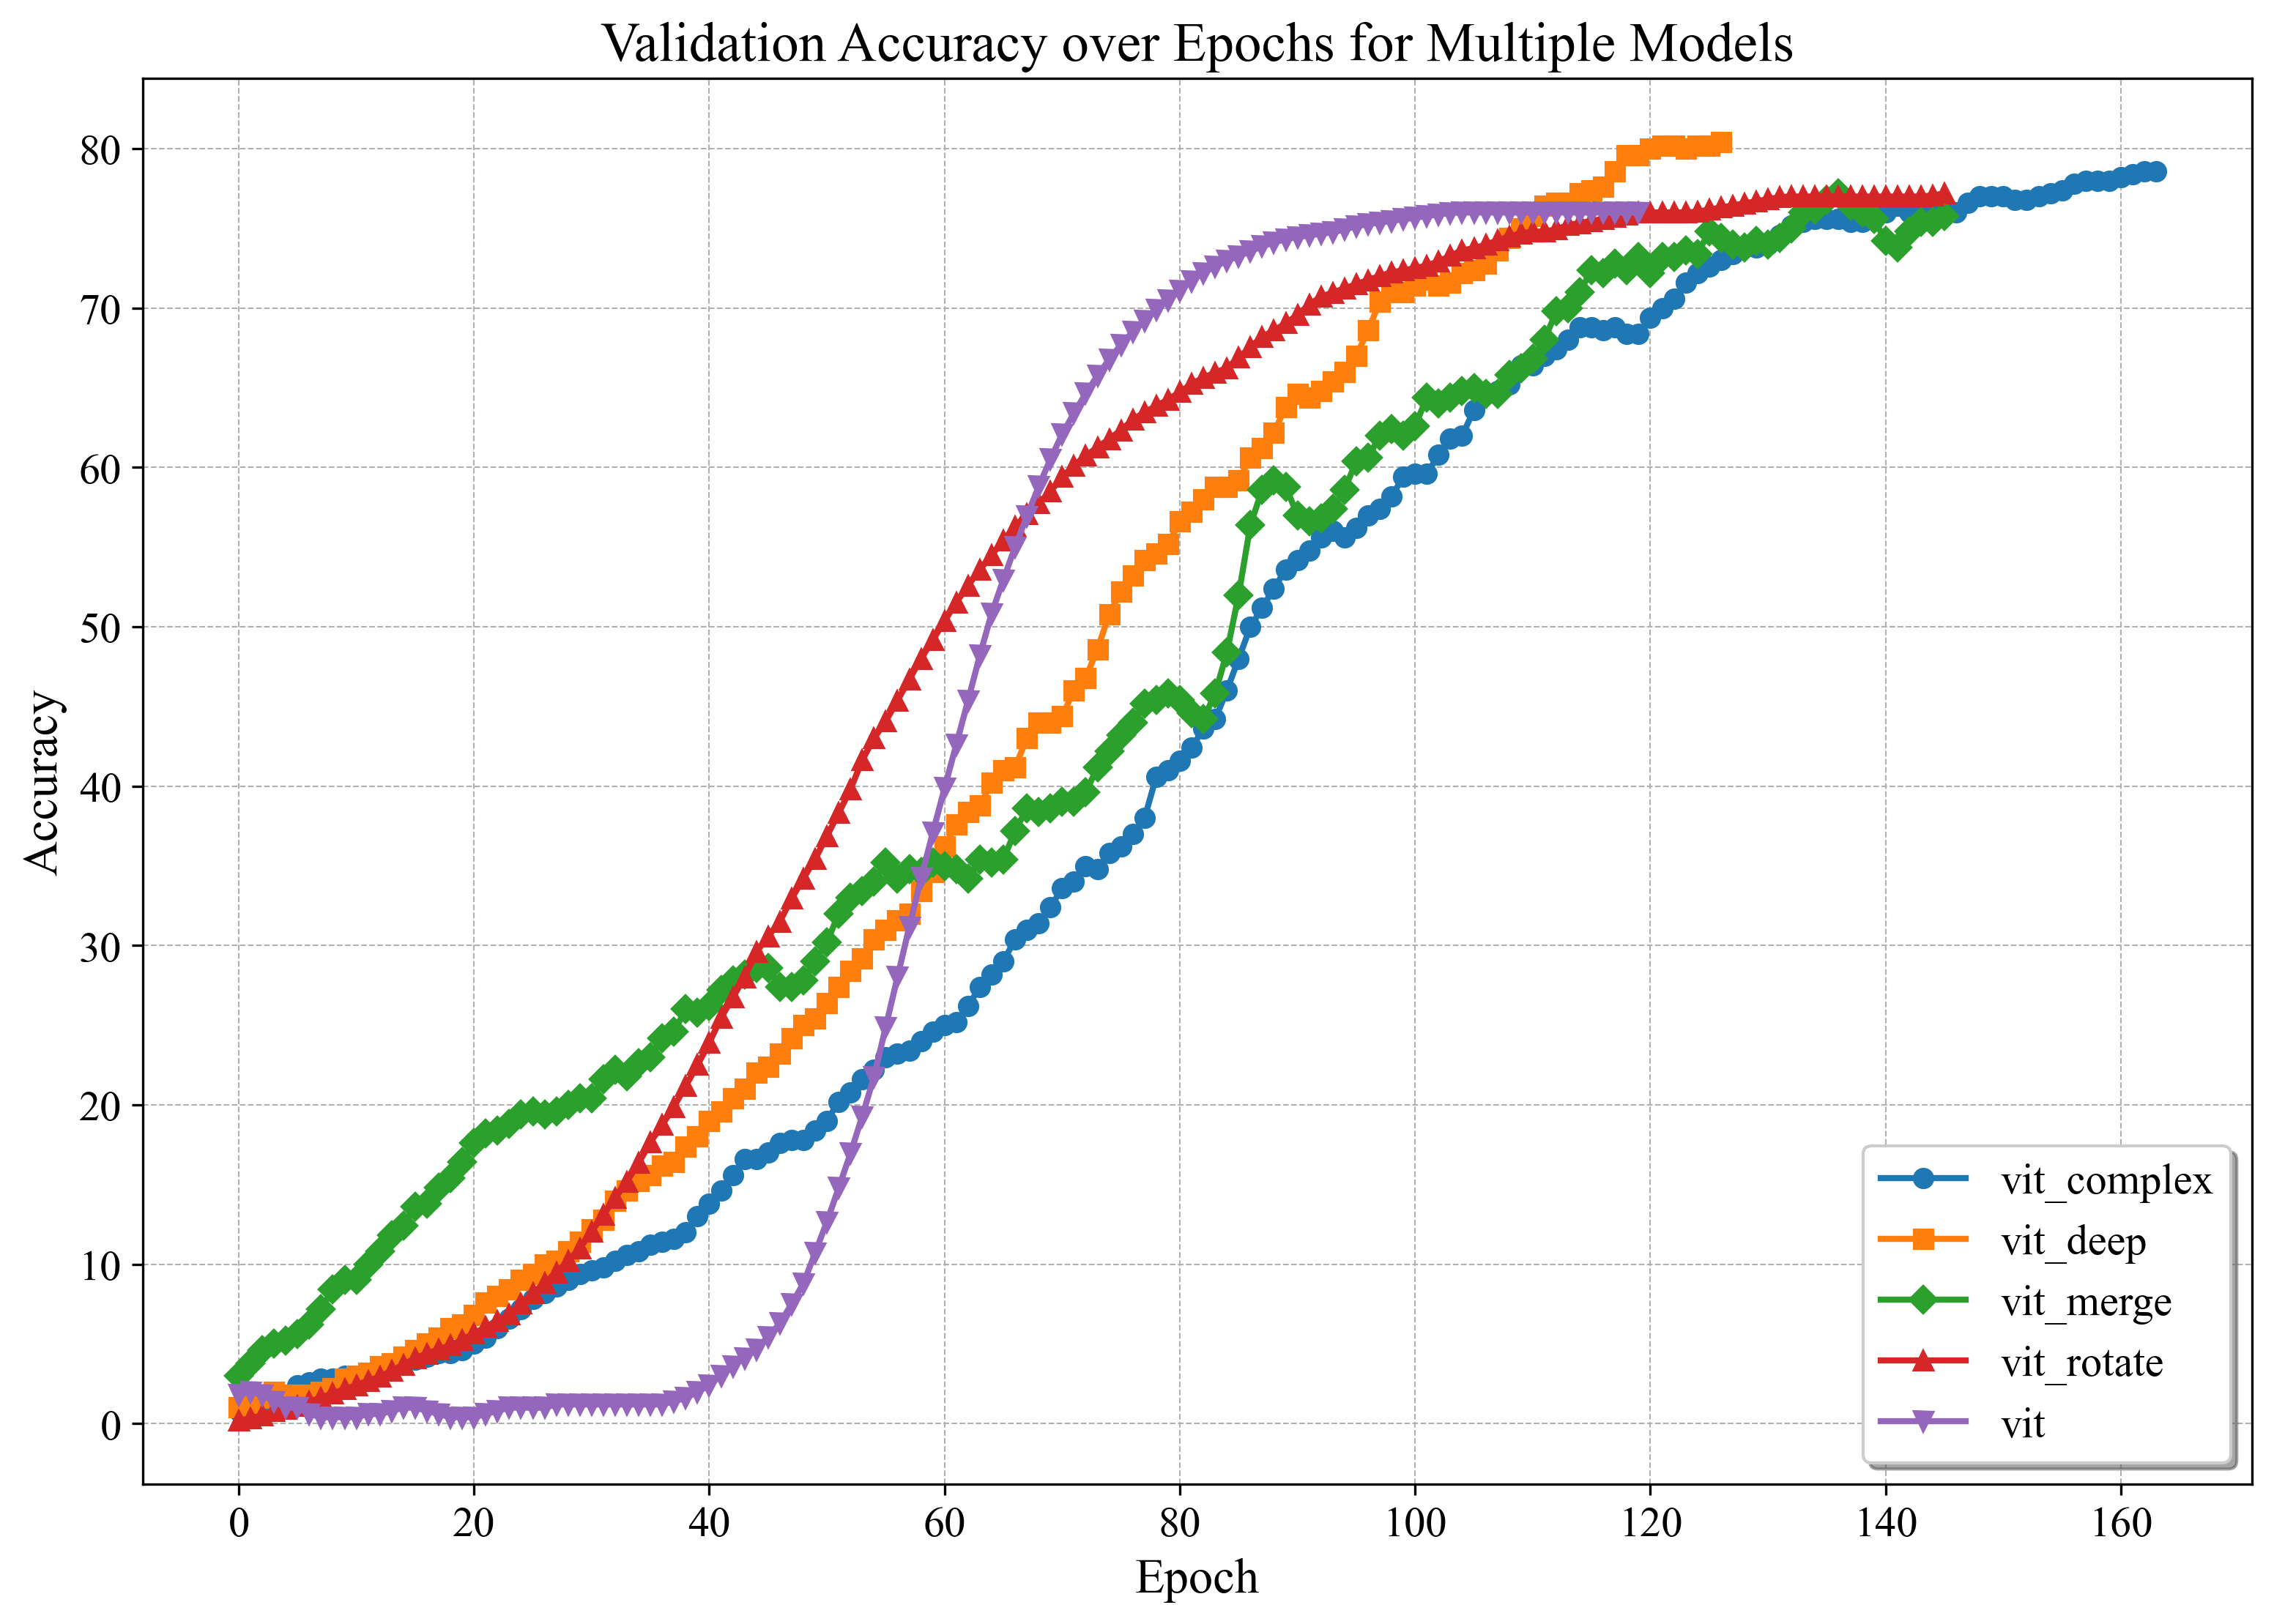
\includegraphics[width=\textwidth]{figures/Fig4.png}
        \caption{Validation Accuracy over Epochs for Multiple ViT Models.}
        \label{fig:validation_accuracy}
    \end{subfigure}
    \caption{Comparison of Validation Accuracy over Epochs for ViT and PVT Models.}
\end{figure}

\section{Conclusion}

Positional encoding is essential for structuring information in neural networks, with its generality suggesting a unified algorithmic strategy that applies across visual, auditory, and linguistic domains. This study introduces GridPE, a unified framework inspired by grid cells in the mammalian brain, to enhance transformer architectures for high-dimensional data processing. GridPE captures both absolute and relative positioning, crucial for tasks involving spatial relationships. Experiments in image classification demonstrate that GridPE achieves competitive accuracy compared to state-of-the-art approaches. Its versatility and scalability across different data domains suggest promising applications in natural language processing, robotics, and spatial cognition, blending neuroscience principles with artificial intelligence.

\bibliography{aaai25}

% \section{Reproducibility Checklist}

% \textbf{This paper}
% \begin{itemize}
%     \item Includes a conceptual outline and/or pseudocode description of AI methods introduced: \textbf{yes}
%     \item Clearly delineates statements that are opinions, hypothesis, and speculation from objective facts and results: \textbf{yes}
%     \item Provides well marked pedagogical references for less-familiar readers to gain background necessary to replicate the paper: \textbf{yes}
%     \item Does this paper make theoretical contributions? \textbf{yes}
%     \begin{itemize}
%         \item All assumptions and restrictions are stated clearly and formally: \textbf{yes}
%         \item All novel claims are stated formally (e.g., in theorem statements): \textbf{yes}
%         \item Proofs of all novel claims are included: \textbf{yes}
%         \item Proof sketches or intuitions are given for complex and/or novel results: \textbf{yes}
%         \item Appropriate citations to theoretical tools used are given: \textbf{yes}
%         \item All theoretical claims are demonstrated empirically to hold: \textbf{yes}
%         \item All experimental code used to eliminate or disprove claims is included: \textbf{yes}
%     \end{itemize}
%     \item Does this paper rely on one or more datasets? \textbf{yes}
%     \begin{itemize}
%         \item A motivation is given for why the experiments are conducted on the selected datasets: \textbf{yes}
%         \item All novel datasets introduced in this paper are included in a data appendix: \textbf{NA}
%         \item All novel datasets introduced in this paper will be made publicly available upon publication of the paper with a license that allows free usage for research purposes: \textbf{NA}
%         \item All datasets drawn from the existing literature (potentially including authors’ own previously published work) are accompanied by appropriate citations: \textbf{yes}
%         \item All datasets drawn from the existing literature (potentially including authors’ own previously published work) are publicly available: \textbf{yes}
%         \item All datasets that are not publicly available are described in detail, with explanation why publicly available alternatives are not scientifically satisficing: \textbf{NA}
%     \end{itemize}
%     \item Does this paper include computational experiments? \textbf{yes}
%     \begin{itemize}
%         \item Any code required for pre-processing data is included in the appendix: \textbf{yes}
%         \item All source code required for conducting and analyzing the experiments is included in a code appendix: \textbf{yes}
%         \item All source code required for conducting and analyzing the experiments will be made publicly available upon publication of the paper with a license that allows free usage for research purposes: \textbf{yes}
%         \item All source code implementing new methods have comments detailing the implementation, with references to the paper where each step comes from: \textbf{yes}
%         \item If an algorithm depends on randomness, then the method used for setting seeds is described in a way sufficient to allow replication of results: \textbf{NA}
%         \item This paper specifies the computing infrastructure used for running experiments (hardware and software), including GPU/CPU models; amount of memory; operating system; names and versions of relevant software libraries and frameworks: \textbf{yes}
%         \item This paper formally describes evaluation metrics used and explains the motivation for choosing these metrics: \textbf{yes}
%         \item This paper states the number of algorithm runs used to compute each reported result: \textbf{yes}
%         \item Analysis of experiments goes beyond single-dimensional summaries of performance (e.g., average; median) to include measures of variation, confidence, or other distributional information: \textbf{no} — The paper focuses on key performance metrics without including variation or confidence measures.
%         \item The significance of any improvement or decrease in performance is judged using appropriate statistical tests (e.g., Wilcoxon signed-rank): \textbf{no} - Statistical tests were not used, as the paper emphasizes comparative analysis rather than hypothesis testing.
%         \item This paper lists all final (hyper-)parameters used for each model/algorithm in the paper’s experiments: \textbf{partial} - General hyperparameters are provided, but not exhaustively listed for each model.
%         \item This paper states the number and range of values tried per (hyper-) parameter during development of the paper, along with the criterion used for selecting the final parameter setting: \textbf{partial} - The paper outlines general criteria for hyperparameter selection but does not detail all values tested.
%     \end{itemize}
% \end{itemize}

\end{document}
